% Ein Beispielkapitel
%

\chapter{Basics}

\section{Analog to digital conversion}

Zun�chst referenzieren wir die Abbildung \ref{fig:driver_structure} (mit \verb|\ref{fig:driver_structure}|), die aus dem Buch \cite{Lankes02} (\verb|\cite{Lankes02}|) genommen wurde. Die Tabelle \ref{tab:vergleich} (Referenz erzeugt mit \verb|\ref{tab:vergleich}|) darf nat�rlich nicht fehlen. Fu�noten\footnote{Ich bin eine Fu�note} (erzeugt mit \verb|\footnote{Ich bin eine Fu�note}|) k�nnen ebenfalls verwendet werden. Und im Quelltext sieht ein Indexeintrag mit Ober- und Unterbegriff folgenderma�en aus: \index{Oberbegriff!Unterbegriff}\verb|\index{Oberbegriff!Unterbegriff}|.

\begin{figure} %[htbp] %hier k�nnen noch Positionierungsw�nsche angegeben werden
	\centering   % Alles weitere zentrieren
	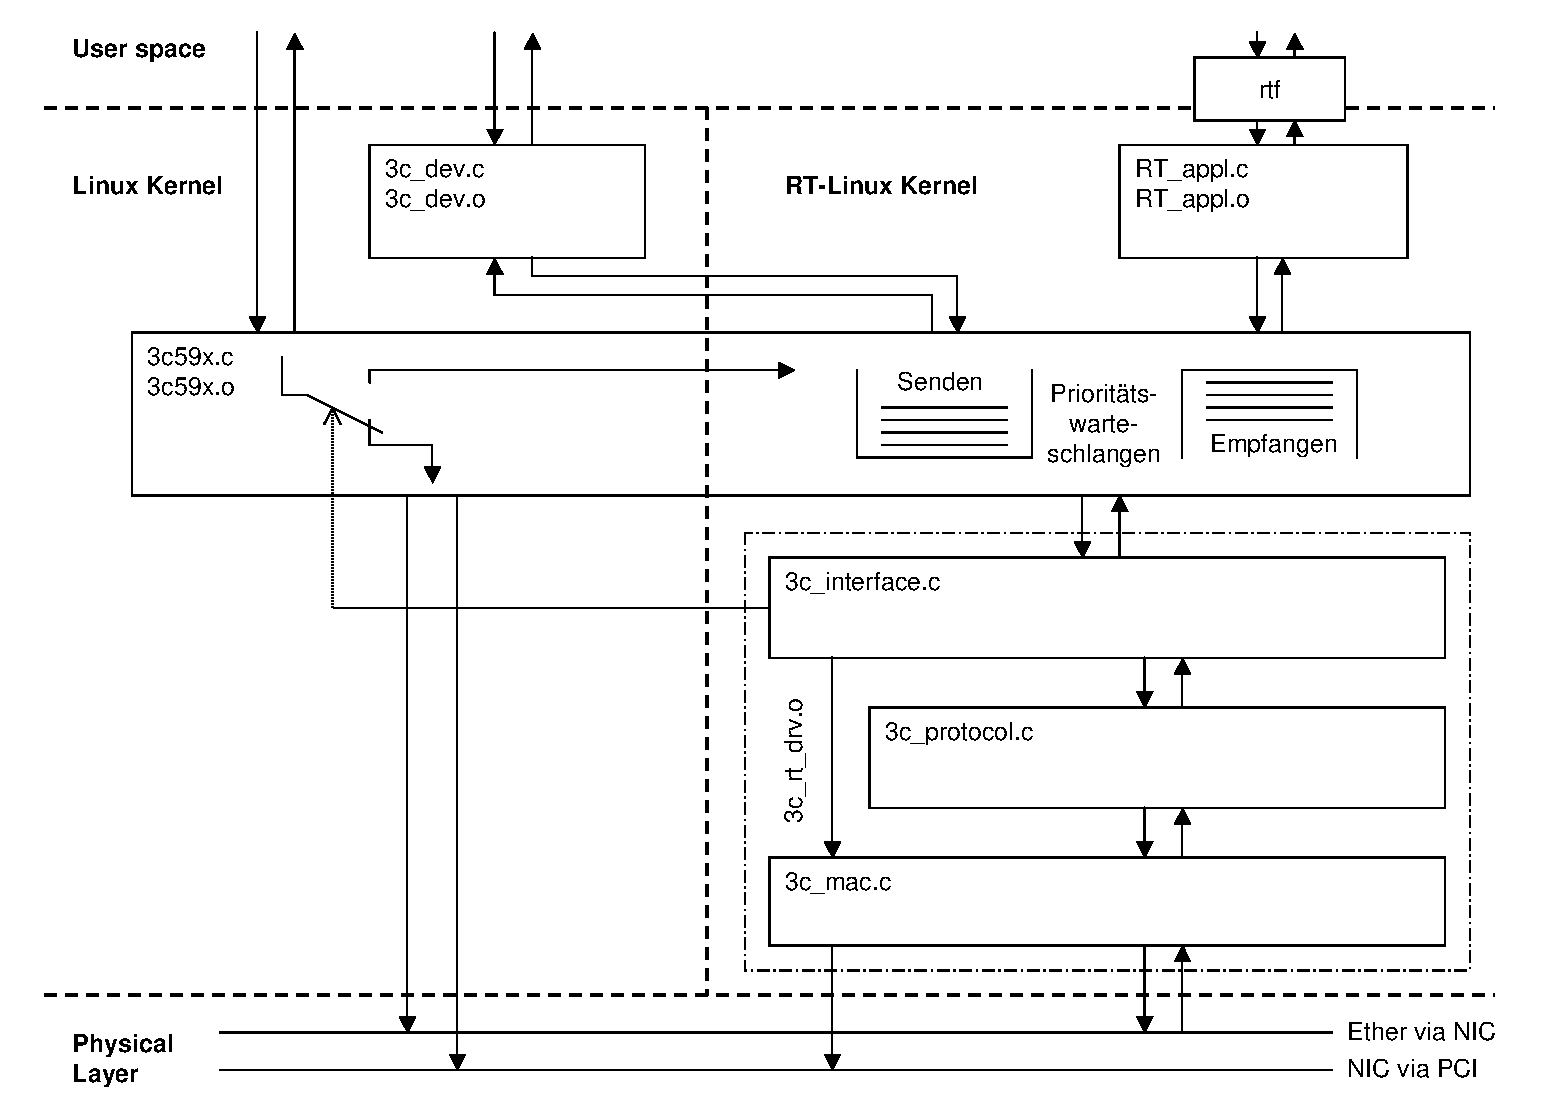
\includegraphics[width=13cm]{pictures/treiberstruktur}
	\caption{Treiberstruktur des zeitgesteuerten\index{Allgemein!Realzeit|(} Ethernet (verschiebbare Grafik)}
	\label{fig:driver_structure}  %Reihenfolge ist wichtig! Immer erst \caption{} dann \label{}
\end{figure}


\begin{table} %[htbp] %hier k�nnen noch Positionierungsw�nsche angegeben werden
	\centering      % Alles weitere zentrieren
	\begin{tabular}{|c|c|c|c|} %Alle Spalten zentrieren, ansonsten 'r' oder 'l'
		\hline
		\textbf{Item}   & \textbf{Multi-}    & \textbf{Multi-}   & \textbf{Distributed} \\
		                & \textbf{processor} & \textbf{computer} & \textbf{System}      \\
		\hline \hline
		node            & CPU                & CPU, RAM,         & complete             \\
		configuration   &                    & net interface     & computer             \\
		\hline
		node peripherie & all shared         & shared exc.       & full set             \\
		                &                    & maybe disk        & per node             \\
		\hline
		location        & same rack          & same room         & possibly             \\
		                &                    &                   & worldwide            \\
		\hline
		internode       & shared RAM         & dedicated         & traditional          \\
		communication   &                    & interconnect      & network              \\
		\hline
		operating       & one, shared        & multiple, same    & possibly all         \\
		system          &                    &                   & different            \\
		\hline
		file systems    & one, shared        & one, shared       & each node has own    \\
		\hline 
		administration  & one organization   & one organization  & many organizations   \\
		\hline
	\end{tabular}
	\caption{Vergleich der verschiedenen Systemen (verschiebbare Tabelle)}
	\label{tab:vergleich}  %Reihenfolge ist wichtig! Immer erst \caption{} dann \label{}
\end{table}

\section{Abschnitt mit ortsfester Tabelle und Grafik}

Eigentlich sollten ortsfeste Objekte nur sehr selten genutzt werden,
nichtsdestotrotz wird in diesem Abschnitt kurz gezeigt, wie man Grafiken und 
Tabellen ordentlich nummeriert und referenziert, obwohl sie nicht in eine 
\emph{figure} oder \emph{table} Umgebung eingebettet sind. Diese Art der
Einbindung erlaubt volle Kontrolle �ber die Platz\-ier\-ung der eingebundenen
Objekte.

\textbf{\emph{Hinweis:} Allerdings kann es passieren, dass die Floats hinter die
non-Floats verschoben werden und somit die Nummerierung "`falsch herum"'
vorgenommen wird.}

Hier werden wir einfach das Lehrstuhl-Logo \ref{fig:Logo} noch einmal genau
unter dieser Zeile einblenden:

\begin{nffigure} %Non-Floating Figure einbinden
	\centering
	
\includegraphics[width=12.2cm]{logo/LfBS_LOGO_3c}
	\caption{Unser Lehrstuhl-Logo}
	\label{fig:Logo}  %Reihenfolge ist wichtig! Immer erst \caption{} dann \label{}
\end{nffigure}

Mit Tabellen funktioniert das ganz genau so (siehe \ref{tab:Testtabelle}):

\begin{nftable} %Non-Floating Table einbinden
	\centering
	\begin{tabular}{|c|c|c|}
		\hline
		Test1 & Test2 & Test3\\
		\hline
		Test4 & Test5 & Test6\\
		\hline
	\end{tabular}
	\caption{Eine ortsfeste Testtabelle}
	\label{tab:Testtabelle}  %Reihenfolge ist wichtig! Immer erst \caption{} dann \label{}
\end{nftable}
